\chapter{Approksimationsalgoritmer}

\section{Set-Cover Problemet}%
\label{sec:SetCover}

\textsc{Set-Cover} problemet, siger, at givet et input $(X, \mathcal{F})$, hvor $X$ er en endelige mængde og $\mathcal{F}$ er en familie af delmængder af $X$, så find en delmængde $\mathcal{F}'$ af $\mathcal{F}$, således at $\bigcup_{S \in \mathcal{F}'} S = X$, hvor $|\mathcal{F}|$ er minimeret.

\begin{wrapfigure}{r}{0.5\textwidth}
	\centering
	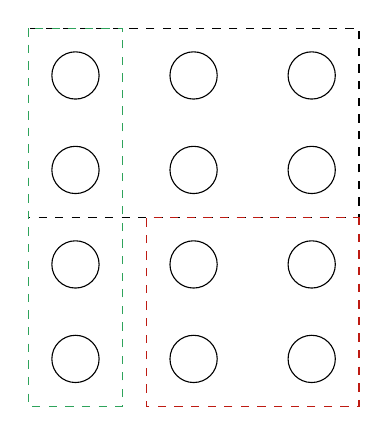
\begin{tikzpicture}[scale=1.2]
		\draw  (7.25,15) circle (0.25cm);
		\draw  (7.25,14) circle (0.25cm);
		\draw  (7.25,13) circle (0.25cm);
		\draw  (7.25,12) circle (0.25cm);
		\draw  (8.5,15) circle (0.25cm);
		\draw  (8.5,14) circle (0.25cm);
		\draw  (8.5,13) circle (0.25cm);
		\draw  (8.5,12) circle (0.25cm);
		\draw  (9.75,15) circle (0.25cm);
		\draw  (9.75,14) circle (0.25cm);
		\draw  (9.75,13) circle (0.25cm);
		\draw  (9.75,12) circle (0.25cm);
		\draw [, dashed] (6.75,15.5) rectangle  (10.25,13.5);
		\draw [ color={rgb,255:red,46; green,163; blue,91} , dashed] (6.75,15.5) rectangle  (7.75,11.5);
		\draw [ color={rgb,255:red,190; green,27; blue,19} , dashed] (10.25,13.5) rectangle  (8,11.5);
	\end{tikzpicture}
	\caption{\label{fig:setcover} Et eksempel på en løsning af et Setcover Problem hvor $|\mathcal{F}'| = 3$}
\end{wrapfigure}

I Figur~\ref{fig:setcover} ses et eksempel på en løsning af en instans af set-cover problemet, hvor $|\mathcal{F}'| = 3$. Bemærk dog at delmængderne i $\mathcal{F}'$ ikke behøver at have den form, de skal bare være normale delmængder.

Optimiseringsversionen af \textsc{Vertex-Cover} er et specielt case af \textsc{Set-Cover}, hvilket betyder, at når vi ved at \textsc{Vertex-Cover} problemet er svært at løse, så er \textsc{Set-Cover} også. Vi transformerer fra \textsc{VC} til \textsc{SC} som følger: Givet en graf $G = (V,E)$, konstruer en instans $(X, \mathcal{F})$ af \textsc{Set-Cover} problemet. Lad $X = E$ og $\mathcal{F} = \{S_{v} \mid v \in V\}$, hvor $S_{v}$ er mængden af kanter som $v$ ``dækker''. Dette er en reduktion, så dermed, siden decision versionen af \textsc{Vertex-Cover} er NP-komplet, så er decision versionen af \textsc{Set-Cover}, som tager en instans $(X, \mathcal{F}, k)$ og spørger om det er muligt at ``dækker'' alle mængder med højest $k$ delmængder. delmængder.

I Algoritme~\ref{alg:greedysetcover} ses en grådig algoritme som finder et cover. I algoritmen er variablen $Z$ de elementer der endnu ikke er dækket, og $\mathcal{F}'$ er delmængderne som dækker den del af $X$ der er dækket, altså $\hat{Z}$. Løkken vælger en delmængde i $\mathcal{F}$ som dækker flest mulige nye elementer. Bemærk dog, at algoritmen antager at det er muligt at dækker alle elementer i $X$, altså $\bigcup_{s \in \mathcal{F}} s = X$.

\begin{algorithm}
	\caption{\label{alg:greedysetcover}Grådig Set Cover}
	\begin{algorithmic}
		\REQUIRE $X$, $\mathcal{F}$
		\STATE $Z \leftarrow X$
		\STATE $\mathcal{F}' \leftarrow \emptyset$
		\WHILE{$Z \neq \emptyset$}
		\STATE Vælg $S \in \mathcal{F}$ således at $|S \cap Z|$ er maksimeret.
		\STATE $Z \leftarrow Z \setminus S$
		\STATE $\mathcal{F}' \leftarrow \mathcal{F}' \cup \{S\}$
		\ENDWHILE
		\RETURN $\mathcal{F}'$
	\end{algorithmic}
\end{algorithm}

\begin{theorem}
	Den grådige set-cover algoritme er en $H(|X|)$-approksimationsalgoritme.
\end{theorem}
\begin{proof}
	Husk at $\sum_{i=1}^n \frac{1}{i} = H(n)$. Vi ser på mængden af delmængder vi vælger til set-coveret som værende $\mathcal{F}' = \{S_{1}, S_{2}, \ldots, S_{|\mathcal{F}'|}\}$, hvor $S_{|\mathcal{F}'|}$ er den sidste delmængde, og den der dækker de resterende elementer.

	$\forall x \in X$: Lad $S_{i}$ være den første mængde i $\mathcal{F}'$ som indeholder $x$ og tildel $x$ \textit{vægten} $c_{x} = \frac{1}{|S_{i} \setminus (S_{1} \cup \cdots \cup S_{i-1})|}$. Altså kan man se på vægten som værende $\frac{1}{x}$ hvor $x$ er antallet af nye elementer dækket af $S_{i}$. Dermed vil hvert element i en delmængde der dækker 10 nye elementer have vægt $\frac{1}{10}$. Hvis man summerer vægten for hvert element i grafen, får man antallet af delmængder i løsningen $\mathcal{F}'$. For eksempel, hvis en delmængde dækker 20 elementer i alt, og af disse 20 er 10 af elementerne ikke dækket får, så får hvert element vægt $\frac{1}{10}$ og når vi summerer den nydækkede del får vi $\frac{1}{10} \cdot 10 = 1$. Dermed får vi ligningen $|\mathcal{F}'| = \sum_{x \in X} c_{x}$.

	Vi vil nu estimere hvor langt fra det optimale vi er. Lad $\mathcal{F}^{*}$ være den optimale familie af delmængder.
	\begin{equation}
		\label{eq:flessthanoptimal}
		|\mathcal{F}'| = \sum_{x \in X}^n \le \sum_{S \in \mathcal{F}^{*}} \sum_{x \in S} c_{x}
	\end{equation}

	Uligheden i~\ref{eq:flessthanoptimal} kommer fra, at vi beholder værdien på hvert element, $c_{x}$; som nu muligvis er i mere end en delmængde fra $\mathcal{F}$. Dermed vil den muligvis også blive tællet mere end én gang.

	\begin{claim}
		\label{claim:costlessthanharmonic}
		\begin{equation*}
			\forall S \in \mathcal{F}	\;	\sum_{x \in S} c_{x} \le H(|S|)
		\end{equation*}
	\end{claim}
	Hvis vi antager påstand~\ref{claim:costlessthanharmonic} til at være korrekt, får vi følgende resultat:
	\begin{align*}
		|\mathcal{F}'| \le \sum_{s \in \mathcal{F}^{*}} \sum_{x \in S} c_{x} & \le \sum_{s \in \mathcal{F}^{*}} H(|S|)                          \\
		                                                                     & \le \sum_{S \in \mathcal{F}^{*}} H(\max_{S \in \mathcal{F}} |S|) \\
		                                                                     & \le \sum_{s \in \mathcal{F}^{*}} H(|X|)                          \\
		                                                                     & = |\mathcal{F}^{*}| H(|X|)
	\end{align*}
	Dette viser at den grådige algoritme er en $H(|X|)$-approksimationsalgoritme.
\end{proof}

Vi vil nu bevise påstand~\ref{claim:costlessthanharmonic}.

\begin{proof}
	Vi kigger på en arbitrær fastsat $S \in \mathcal{F}$ og lader $k$ være en konstant således at $S \not \subseteq S_{1} \cup \cdots \cup S_{k-1}$ men $S \subseteq S_{1} \cup \cdots \cup S_{k}$.

	Lad $u_{i} = |S \setminus S_{1} \cup \cdots \cup S_{i}|$ for $i = 0,1, \ldots, k$. Altså kan $u_{i}$ defineres til at være antallet af elementer som endnu ikke er dækket af delmængderne $S_{1} \cup \cdots \cup S_{i}$. Ud fra denne definition er det klart at se at $u_{0} = |S|$, $u_{k} = 0$, og $u_{i-1} \ge u_{i}$. Vi kan ud fra dette også se at $u_{i-1} - u_{i}$ er antallet af nye elementer af $S$ som dækkes af $S_{i}$.

	Derudover gælder det at $|S_{i} \setminus (S_1 \cup \cdots \cup S_{i-1})| \ge |S \setminus (S_{1} \cup \cdots \cup S_{i-1})|$ da $A$ vælger $S_{i}$ i skridt $i$.

	Så:
	\begin{align*}
		\sum_{x \in S} c_{x} & = \sum_{i=1}^k (u_{i-1}-u_{i}) \cdot \frac{1}{|S_{i} \setminus (S_{1} \cup \cdots \cup S_{i-1})|} \\
		                     & \le \sum_{i=1}^k  (u_{i-1}-u_{i}) \cdot \frac{1}{|S \setminus (S_{1} \cup \cdots \cup S_{i-1})|}  \\
		                     & \le \sum_{i=1}^k \frac{u_{i-1}-u_{i}}{u_{i-1}}
	\end{align*}
	Ved den første linje, er $(u_{i-1}-u_{i})$ antallet af nye elementer som $S_{i}$ dækker. $\frac{1}{|S_{i} \setminus (S_{1} \cup \cdots \cup S_{i-1})|}$ er 1 over antallet af nye elementer dækket, altså det samme som prisen $c_{x}$ for et element $x \in S_{i}$. Dermed, ved at vi summerer alle $S_{i}$ får vi det samme som $\sum_{x \in S} c_{x}$, som summerer igennem alle elementer i $S$.


	Bemærk at når $b \ge a$ gælder følgende:
	\begin{equation*}
		H(b)-H(a) = \sum_{i=a+1}^b \frac{1}{i} \ge (b-a) \cdot \frac{1}{b}
	\end{equation*}

	Dermed får vi følgende:
	\begin{align*}
		\sum_{x \in S} c_{x} & \le \sum_{i=1}^k \frac{u_{i-1}-u_{i}}{u_{i-1}} \\
		                     & \le \sum_{i=1}^k (H(u_{i-1})-H(u_i))           \\
		                     & = H(u_{0}) - H(u_{k})                          \\
		                     & = H(u_{o})                                     \\
		                     & = H(|S|)
	\end{align*}
	Husk at $H(u_{k}) = 0$.
	Ud fra disse udregninger får vi $\sum_{x \in S} c_{x} \le H(|X|)$.
\end{proof}

Undtagen hvis $P = NP$, er det ikke muligt at finde en bedre approksimationsalgoritme for \textsc{Set-Cover}. Approksimationsfaktoren er altså $o(\log |X|)$.

\section{Randomisering og Lineær Programmering}%
\label{sec:randomizationandlp}

Husk at en indicator random variabel er en variabel hvis værdi enten er $1$ eller $0$:
\begin{equation*}
	X_{A}(s) = \begin{cases}
		1 & \text{ hvis } s \in A    \\
		0 & \text{ hvis } s \notin A
	\end{cases}
\end{equation*}
En randomiseret approximationsalgoritme $A$ er en \(\rho\)-approximationsalgoritme hvis $\max \left( \frac{C}{C^{*}}, \frac{C^{*}}{C} \right) \le \rho$ når $C$ er \textbf{den forventede værdi} af løsningen fundet af $A$.

\subsection{Max-3-SAT}%
\label{subsec:label}

\textsc{Max-3-SAT} (Som set i DM551) tager en instans af \textsc{3-SAT} $\mathcal{F} = C_{1} \wedge C_{2} \wedge \cdots \wedge C_{m}$ over variabler $x_{1}, x_{2}, \ldots, x_{n}$, og finder en sandhedstildeling $\phi : \{x_{1}, x_{2}, \ldots, x_{n}\} \rightarrow \{T, F\}^{n}$ som maksimerer antallet af satisfied klausuler.

Algoritme~\ref{alg:randomiseret3sat} viser hvordan en randomiseret algoritme kan løse problemet.
\begin{algorithm}
	\caption{\label{alg:randomiseret3sat}Randomiseret Algoritme $A$}
	\begin{algorithmic}[1]
		\FOR{$i := 1 \to n$}
		\STATE giv $x_i$ værdi T (sand) med sandsynlighed $\frac{1}{2}$
		\STATE giv $x_{i}$ værdi F (falsk) med sandsynlighed $\frac{1}{2}$
		\ENDFOR
	\end{algorithmic}
\end{algorithm}

Selve de randomiseret algoritmer er ofte ekstremt simple; det svære er deres analyse. Vi vil nu analysere Algoritme~\ref{alg:randomiseret3sat}. Lad den tilfældige variabel $X$ være antallet af satisfied klausuler af $A$. Så er $X = X_{1} + X_{2} + \cdots + X_{m}$, hvor
\begin{equation*}
	X_{i} = \begin{cases}
		1 & \text{ hvis }C_{i} \text{ er satisfied af }A \\
		0 & \text{ ellers}
	\end{cases}
\end{equation*}
Sandsynligheden for $P(X_i = 1) = 1 - P(X_{i} = 0) = 1 - (\frac{1}{2})^{3} = \frac{7}{8}$. Den forventede værdi af en indicator random variable er blot sandsynligheden for at dens resultat er $1$. Dermed $E(X_i) = \frac{7}{8}$. Ved linearity of expectation, kan vi finde den forventede værdi for at alle klausuler bliver satisfied:
\begin{equation*}
	C = E(X) = E(\sum_{i=1}^m X_{i}) = \sum_{i=1}^m E(X_{i}) = \sum_{i=1}^m \frac{7}{8} = \frac{7m}{8}
\end{equation*}

Her får vi så:
\begin{equation*}
	\frac{C^{*}}{C} \le \frac{m}{\frac{7m}{8}} = \frac{8}{7} \le \rho
\end{equation*}

Dermed er $A$ en randomiseret $\frac{7}{8}$-approximationsalgoritme til \textsc{Max-3-SAT}.

\subsection{Vægtet Vertex-Cover}%
\label{subsec:weightedvertexcover}

Givet en graf $G = (V,E)$ og en vægtfunktion $w : V \rightarrow \mathbb{R}_{+}$, find et vertex cover $U^{*}$ således at $w(U^{*}) \le w(U)$, hvor $U$ er \textbf{alle} andre vertex covers. Prisen af en mængde $X$ af knuder udregnes $w(X) = \sum_{v \in X} w(v)$. En $\mathcal{NP}$ version af dette problem gives som følger: Givet en graf $G = (V,E), w : V \rightarrow \mathbb{R}_{+}$ og $K \in \mathbb{R}_{+}$, bestem om der eksisterer et vertex cover $u$ hvor $w(u) \le K$. Dette problem er $\mathcal{NP}$-komplet, da det kan reduceres fra \textsc{Vertex-Cover} problemet, ved at tage $w(v) = 1\; \forall v \in V$.

Vi kan formulere \textsc{Weighted-Vertex-Cover} problemet som et 0-1 heltals programmeringsproblem. Vi definerer $X(v)$ til  at være $1$, hvis og kun hvis $v \in U$, altså $X(v) = 1 \iff v \in U$. Hvis $X(v) \ne 1$, så $X(v) = 0$ (i og med det er et 0-1 heltals programmeringsproblem). Vores tilstand er at $\forall (u,v) \in E \mid X(u) + X(v)  \ge 1 $, altså skal mindst én knude i hver kant have værdi $X(v) = 1$. Vores mål er $\min \sum_{v \in V} X(v) w(v) $, altså at finde det billigste mulige cover.

\begin{equation*}
	Z_{I} = \text{opt} = \min \sum_{v \in V} X(v) w(v)
\end{equation*}

Vi kan løse dette ved, fremfor at lade $X(u) \in \{0,1\}\; \forall u \in V$, så lader vi $0 \le X(u) \le 1$. Her bruger vi \textit{lineær programmering}, som er polynomielt. Vi bruger \textit{LP-Relaxation} metoden, som er metoden der tillader $X(u)$ til at have værdier mellem, og inklusiv, 0 og 1.
\begin{align*}
	Z_{LP}        & = \min \sum_{v} x(v) \cdot w(v)           \\
	\Delta	 \quad & x(u) + x(v) \geq 1 \quad \forall uv \in E \\
	              & 0 \leq x(v) \leq 1 \quad \forall v \in V
\end{align*}

Ved at bruge LP-relaxation, får vi en løsning hvor $Z_{LP} \le Z_{I} = \text{opt}$. Algoritme~\ref{alg:approxwvc} bruger lineær programmering til at løse \textsc{Weighted-Vertex-Cover} problemet.

\begin{algorithm}
	\caption{\label{alg:approxwvc}Approximationsalgoritme $B$ for \textsc{Weighted-Vertex-Cover}}
	\begin{algorithmic}[1]
		\STATE Løs LP-relaxation og lad $\bar{x} = (\bar{x}(v))_{v \in V}$ være en optimal løsning til denne.
		\STATE Lad $U = \{v \mid \bar{x}(v) \geq \frac{1}{2}\}$
		\RETURN $U$
		\STATE $U$ er et vertex-cover da $\bar{x}$ satisfier $(\Delta)$.
	\end{algorithmic}
\end{algorithm}

\begin{claim}
	$w(u) \le 2 \cdot \text{optimal}$
\end{claim}

\begin{proof}
	\begin{align*}
		\text{optimal} \ge Z_{LP} & = \sum_{v \in V} \hat{X}(v)w(v)                                      \\
		                          & \ge \sum_{\{ v |\hat{X}(v) \ge \frac{1}{2}\}} \hat{X}(w)w(v)    \\
		                          & \ge \sum_{\{ v |\hat{X}(v) \ge \frac{1}{2}\}} \frac{1}{2} \cdot w(v) \\
		                          & = \frac{1}{2} \sum_{v \in U} w(v) = \frac{1}{2} w(U)                      \\
		                          & \Rightarrow w(U) \le 2 \cdot \text{ optimal}
	\end{align*}
\end{proof}

\subsection{Subset-sum problemet}%
\label{subsec:subsetsumproblem}

\textsc{Subset-Sum} er et problem der, givet en mængde $S = \{x_{1}, x_{2}, \ldots, x_{n}\}, \forall v_{i} \in S, v_{i} \in \mathbb{Z}_{+}$ og $t \in \mathbb{Z}_{+}$, skal udregne om der eksisterer en delmængde $I \subseteq \{1, 2, \ldots, n\}$ således at $\sum_{i \in I}x_{i} = t$. Vi kigger her på \textit{optimiseringsversionen}, der siger at \textbf{find et maksimum} $t^{*} \le t$ hvor $I \subseteq \{1, 2, \ldots, n\}$ med $\sum_{i \in I} x_{i} = t^{*}$.

\begin{definition}[Approksimationsskema]
  Et polynomielt approksimationsskema for et problem $Q$, er en algoritme $A = A(\varepsilon)$ hvor $A$ finder en løsning så er indenfor $(1+\varepsilon)$ af den optimale løsning:
  \begin{equation*}
\max\{\frac{C}{C^{*}}, \frac{C^{*}}{C}\} \le (1+ \varepsilon)
\end{equation*}
$A(\varepsilon)$ kører i tid som er polynomielt i $n(\text{størrelsen af inputtet})$ , men ikke nødvendigvis i $\frac{1}{\varepsilon}$, e.g. $n^{5/\varepsilon}$.
\end{definition}

Et approksimationsskema er fuldt polynomielt hvis det fungerer som i definitionen, men $A(\varepsilon)$ er et polynomie i \textbf{både} $n$ og $\frac{1}{\varepsilon}$, e.g. $\left( \frac{1}{\varepsilon} \right)^{6}n^{3}$.

Vi kan nemt løse \textsc{Subset-Sum} problemet i eksponentiel tid. Givet $S = \{x_{1}, \ldots, x_{n}\}$ med $x_{1} \le x_{2} \le \cdots \le x_{n}$, lad $S_{i} = \{x_{1}, \ldots, x_{i}\}, i = 0, 1, \ldots, n$. $L_{i} = $ mængden af heltal vi kan lave som en sum af nogle elementer fra $S_{i}$. $L_{0} = 0, L_{1} = \{0, x_{1}\}, L_{2} = \{0, x_{1}, x_{2}, x_{1}+x_{2}\}$. For at gå fra $L_{i}$ til $L_{i+1}$ tilføjer vi $x_{i+1}$ til alle tal i $L_{i}$, og fjerner løsninger hvis værdier er større end $t$. Denne liste kan fordoble sig i hvert skridt, så $|L_{n}|$ kan være op til $2^{n}$, hvilket vil sige at algoritmen er eksponentiel. Et eksempel på et problem der fordobler sig i hvert skridt er $S= \{1, 2, 4, 8, 16, \cdots, 2^{n-1}\}$ hvor $t \ge 2^{n}$.

Algoritmen er polynomiel hvis en af følgende gælder:
\begin{enumerate}
  \item $t$ er ``lille'' i som en funktion af $n$.
  \item Alle $x_{i} \le p(n)$ for et polynomie $p$.
\end{enumerate}

Vi beskriver nu en idé til et approksimationsskema. Vi udfører \(\delta\)-trimming af listerne. Det vil sige at vi repræsenterer nogle værdier af mindre værdier. Altså, sletter vi tallet $y$, hvis $\frac{y}{(1+\delta)} \le z \le y$. For eksempel, lad $\delta = \frac{1}{10}$, og givet listen $L = \{0, 10, 11, 12, 15, 17, 18, 20, 24 \cdots\}$, så trimmer vi listen til at blive $L' = \{0, 10, 12, 15, 17, 20, 24, \cdots\}$. Processen er som følger ${10}\cdot{1.1} = 11$, dermed bliver 11 fjernet. $17 \cdot 1.1 = 18.7$, derfor ryger 18.

Den ændret algoritme $A'$ fungerer som tidligere, udntagen, før vi bygger $L_{i+1}$ så trimmer vi $L_i$.

\begin{theorem}
$A'$ er et fuldt polynomielt approksimationsskema for \textsc{Subset-Sum} når vi bruger trim-faktoren $\delta = \frac{\varepsilon}{2n}$, hvor $0 <\varepsilon <1$.
\end{theorem}
\begin{proof}
Vi vil gerne vise at $\frac{y^{*}}{<^{*}} \le (1+ \varepsilon)$ hvor $y^{*}$  er værdien af den optimale løsning og $z^{*}$ er outputtet fra $A'$ (som er det største tal i $L_{n}'$). Hvis vi fjerner værdien $y$ fra $L_{j}$ i skridt $j$, så indeholder $L_{j}'$ stadig en værdi $z$ hvor $\frac{y}{(1+\delta)} \le z \le y$. Hvis $z$ senere fjernes i skridt $j' > j$, så er $z$ repræsenteret i $L_{j'}'$  af en værdi $z'$ hvor $\frac{z}{(1+\delta)} \le z'$.

Herfra får vi følgende:
\begin{equation*}
z' \ge \frac{z}{(1+\delta)} \ge \frac{\frac{y}{1+\delta}}{1+\delta} = \frac{y}{(1+\delta)^{2}}.
\end{equation*}
Altså i den sidste iteration er $y^{*}$ repræsentered af et element $z \in L_{n}'$ hvor
\begin{equation}
\frac{y^{*}}{(1+\delta)^{n}} \le z \le y^{*}
\end{equation}
Da $z \in L_{n}'$ er $z \le z^{*}$ hvilket medbærer at $\frac{y^{*}}{(1+\delta)^{n}} \le z \le z^{*}$, så $\frac{y^{*}}{z^{*}} \le (1+\delta)^{n} = (1+ \frac{\varepsilon}{2n})^{n}$. Fra kalkulus ved vi at $(1+ \frac{\varepsilon/2}{n})^{n} \le e^{\varepsilon/2} = 1 + \frac{\varepsilon}{2}+ \left( \frac{\varepsilon}{2} \right)^{2} + \cdots \le 1 + \varepsilon$ når $0 < \varepsilon < 1$. Dermed $\frac{y^{*}}{z^{*}} \le (1+\varepsilon)$. Dermed er $A'$ en $(1+\varepsilon)$-approoksimationsalgoritme.
\end{proof}

Vi vil nu finde køretiden for algoritmen $A'$. Bemærk at $L_{n}'$ altid vil være en variation af $\{0, a_{1}, a_{2}, \ldots, a_{r+1}\}$. $a_{i+1} > \left( 1+ \frac{\varepsilon}{2n} \right)a_{i} \; \forall i$, da $a_{i+1}$ ikke blev fjernet under trimning. Dermed:
\begin{align}
  \left( 1+ \frac{\varepsilon}{2n} \right)^{r} a_{1} &< a_{r+1} \le t \label{l:1}\\
  &\Downarrow\\
  r + \log_{(1+\frac{\varepsilon}{2n})}(a_{1}) &< \log_{\left( 1+ \frac{\varepsilon}{2n} \right)} (t) \label{l:2}\\
  &\Downarrow\\
 r &< \log_{\left( 1 + \frac{\varepsilon}{2n} \right)}  (t) \label{l:3}\\
  &= \frac{\ln t}{\ln \left( 1 + \frac{\varepsilon}{2n} \right) \label{l:4}}
\end{align}

\eqref{l:1} kommer fra at vi mindst skal så langt op for hvert nye element, grundet vores trimningsregler. Vi ved dog også at vi ikke kan komme op til $a_{r+1}$, da den ellers ville have været forsvundet i trimningen. Det er både muligt at $a_{r+1} = t$, men også at den endnu er mindre end $t$. Ved \eqref{l:2} har vi blot puttet logaritmen ind, men base i $1 + \frac{\varepsilon}{2n}$ for at isolere $r$. I ligning \eqref{l:3} fjerner vi $\log_{\left( 1+ \frac{\varepsilon}{2n} \right)}(t)$ fra venstresiden, hvilket giver et svagere argument, men det er stadig mindre end højresiden, som forbliver det samme. Ligning \eqref{l:3} får vi fra at $\log_{a}(x) = \frac{\ln x}{\ln a}$. Så
\begin{align}
  |L_{n}'| = r+2 &< 2 + \frac{\ln t}{\ln (1 + \frac{\varepsilon}{2n})} \label{l:5}\\
 & \le 2 + \frac{2n ( 1 + \frac{\varepsilon}{2n} \ln t)}{\varepsilon} \label{l:6}\\
 & \le 2 + \frac{3n \ln t}{\varepsilon} \label{l:7}\\
 & = 3n \cdot \frac{1}{\varepsilon} \cdot \ln t + 2 \label{l:8}
\end{align}

Ligningen \eqref{l:6} får vi fra \eqref{eq:l6help}.
\begin{equation}
  \label{eq:l6help}
\frac{x}{1+x} \le \ln (1+x) \Rightarrow \frac{1+x}{x} \ge \frac{1}{\ln (1+x)}, x = \frac{\varepsilon}{2n}
\end{equation}

Dette betyder at $A'$ er polynomiel i $n$, $\frac{1}{\varepsilon}$ og $\ln t$.




%%% Local Variables:
%%% mode: latex
%%% TeX-engine: xetex
%%% TeX-command-extra-options: "-shell-escape"
%%% TeX-master: "main"
%%% End:
